\subsection{Complete normalized-smoothness domain across solvers and criteria}
\label{sec:full-s-factorial}
The computational comparison is extended from finite interior penalty grids
to the \emph{entire} normalized smoothness domain
$S\in[0,1]$, with 17 candidate values: eleven deciles
$0,0.1,\ldots,1$ and $0.95,0.99,0.999,0.9999,0.999999,$ and
$0.999999999999$. All numerical algorithms receive \emph{exactly the
same} mapped penalties $\lambda_j=S^{-1}(s_j)$. This preserves the
underlying criterion while permitting a direct test of algebraic
robustness in the high-smoothness tail.

We examine seven backend implementations: fresh and cached dense linear
solves, general banded solves, dense Cholesky, banded Cholesky, symmetric
eigendecomposition, and full SVD. For each, the five statistical criteria
are classical LOOCV, GCV, AICc, BIC and conditional Gaussian profiled
marginal MLE. Difference orders $d=0,1,\ldots,5$ and fixed difference
reference means $\mu=0$ and $\mu=0.15$ are included. The public MLE
model deliberately excludes $d=0$; its combinations are reported
\emph{not applicable}, not scored or imputed.

Two exact limits cannot be treated as ordinary finite factorization
benchmarks. At $S=0$, $\lambda=0$ reproduces the observations, making
standard LOOCV and GCV undefined for the interpolation-only fit. The
marginal likelihood likewise excludes the improper $\lambda=0$
limit. At $S=1$, $\lambda=+\infty$: for $d\geq1$ the fitted trend
is the projection onto the polynomial null space of $D_d$, adjusted
for the fixed $\mu$, whereas for $d=0$ the trend approaches
$\mu\mathbf1$. All solvers share these \emph{analytical} endpoints;
they have no finite Cholesky or LU runtime assigned to them.

For interior penalties, each backend evaluates the complete objective
with its own fit and necessary diagnostics: a conditional leverage
diagonal for LOOCV, EDF for GCV/AICc/BIC, and a properly normalized
determinant/quadratic form or spectral marginal likelihood for MLE.
MLE is not charged for unnecessary CV leverage calculations. Candidate
scores are tested against a spectral reference outside the timed block.
An unstable factorization or an inaccurate score at an extreme finite
penalty is explicitly distinguished from a score that the criterion
defines as infinite. In particular, a short time from an implementation
that fails high-smoothness candidates must \emph{not} be claimed as a
valid whole-grid speed victory.

\begin{figure}[tbp]
\centering
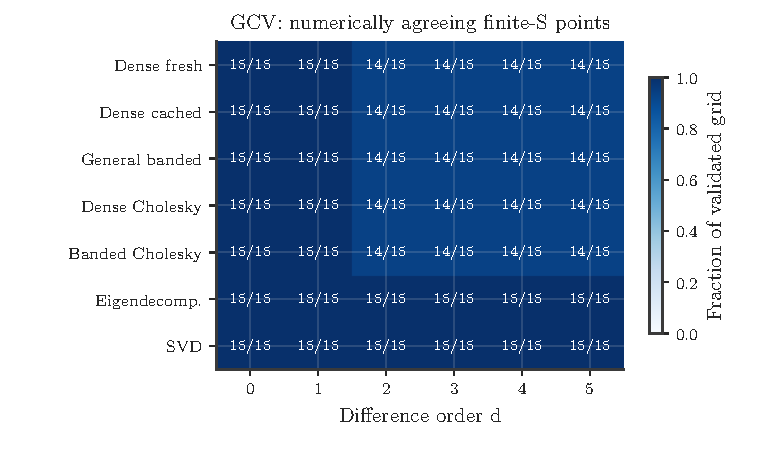
\includegraphics{figures/full_s_validity_gcv.pdf}
\caption{Numerical agreement over all fifteen \emph{finite interior}
normalized-$S$ candidates in an actual GCV selection sweep, for
$n=24$, fixed $\mu=0$, and $d=0,\ldots,5$.
Every heatmap cell shows the number of backend scores agreeing
with the reference out of fifteen; the exact endpoints are handled
analytically. The plot separates arithmetic stability from elapsed
time.}
\label{fig:full-s-validity}
\end{figure}

\begin{figure}[tbp]
\centering
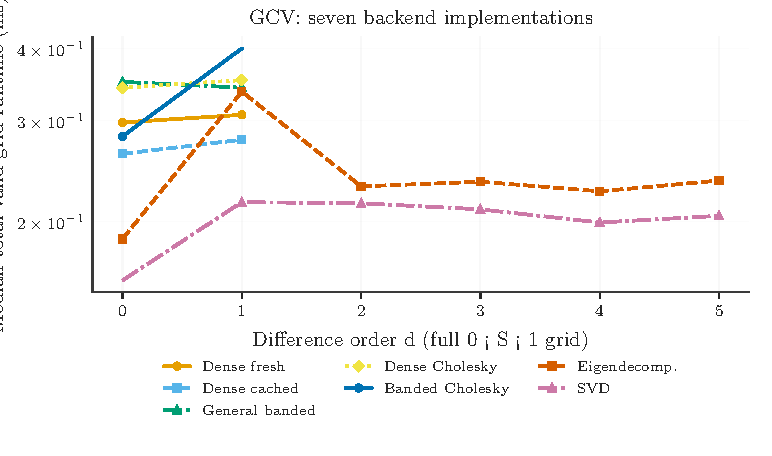
\includegraphics{figures/full_s_time_gcv.pdf}
\caption{Measured total method-specific runtime for an entire
GCV grid, $n=24$, $\mu=0$, and varying difference order.
The cost includes backend preparation and scoring all fifteen
finite interior penalties, with the same $\lambda$ values for each
solver. A backend is \emph{omitted} at a given order if it fails
the numerical agreement or finite-score test for any interior point;
therefore this figure must be read together with
Fig.~\ref{fig:full-s-validity}. The vertical axis is logarithmic.}
\label{fig:full-s-gcv-time}
\end{figure}

\begin{figure}[tbp]
\centering
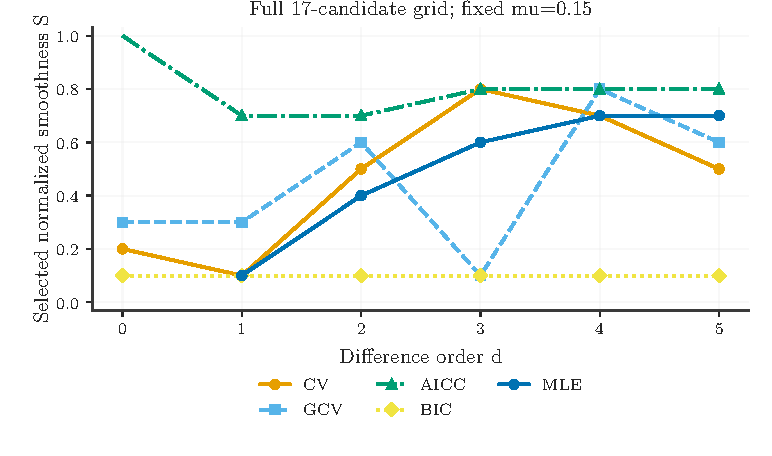
\includegraphics{figures/full_s_selected_mu015.pdf}
\caption{Selected normalized smoothness across all five criterion
definitions and difference orders at fixed nonzero $\mu=0.15$.
Selections are made from the \emph{entire} seventeen-point grid,
including the analytical $S=1$ endpoint. MLE at $d=0$ is not
applicable under the implemented likelihood assumptions.
Selected criterion values are not themselves comparable across
different statistical objectives.}
\label{fig:full-s-selections}
\end{figure}

\begin{figure}[tbp]
\centering
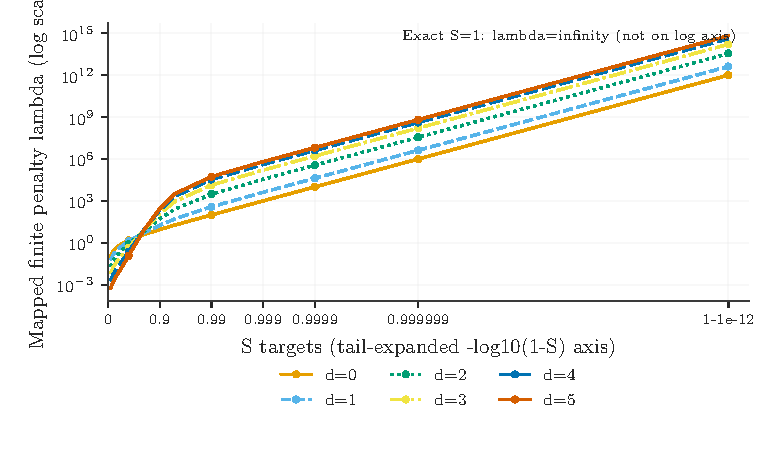
\includegraphics{figures/full_s_lambda_tail.pdf}
\caption{The distinct map $S\mapsto\lambda$ for difference orders
$d=0,\ldots,5$ over the shared near-one candidate grid. The
vertical axis shows only finite positive penalties, on a logarithmic
scale. The \emph{exact} $S=1$ endpoint maps to
$\lambda=+\infty$ and therefore cannot appear on that axis.}
\label{fig:full-s-lambda-tail}
\end{figure}

These exploratory timings are tied to the archived host, random
seed, sample size and repetition counts in
\texttt{paper/benchmarks/full\_s\_reference/environment.json}.
The exhaustive factorial contains all seven solvers, five criteria,
two means and six difference orders, with no invented results for
unsupported or unstable combinations. The full candidate-score matrix,
numerical failures and method-specific timings are stored in
\texttt{candidate\_scores\_and\_times.csv}, the complete-grid
validity and selection outcomes in \texttt{full\_grid\_summary.csv},
and coordinate mappings in \texttt{s\_lambda\_grid.csv}.
The result is a characterization of \emph{conditional in-sample
criteria and numerical implementations}, not evidence of improved
forecast accuracy or a universally fastest backend.
